%\thispagestyle{empty}
\footnotesize
% Setup and stylize appendices to integrate with TOC
\addtocontents{toc}{\protect\renewcommand\protect\cftchappresnum{\appendixname~}}
\renewcommand{\thechapter}{\Roman{chapter}}

% Stylize section header
\renewcommand{\thesection}{\Alph{section}.}

%\addcontentsline{toc}{chapter}{Oligonucleotide and probe sequences}
\chapter{Neural Network Models}
\label{append:two}

\section{Models}
All code\footnote{Code is available at the following url: \url{https://github.com/erickgalinkin/jhu_masters}} was written in Python, using the Tensorflow 2.0, PyTorch, and Scikit-learn libraries.
Only the baseline models described in \ref{other models} used the Scikit-learn library, and only the Wavelet Convolutional network described in \ref{wavelet cnn} used PyTorch.
The remaining models all used the Tensorflow framework.
All models were trained and tested on a 2018 MacBook Pro with 32GB of RAM and a 2.9GHz Intel Core i9 processor.
Given the small size of the data and relative simplicity of the models, GPU acceleration was not needed.
The sections here describe only the details of the architecture.
An overview of the machine learning algorithms is provided in appendix~\ref{append:one}, and a more thorough treatment is available in Hastie~\cite{hastie01statisticallearning} or James~\cite{james14introduction}

\subsection{Standard Fully-Connected Neural Network}
The fully-connected neural network architecture accepts, as input, a 1x100 row-vector.
This vector is then fed to three densely connected layers, each with 256 ReLU-activated neurons.
The output neuron is a single sigmoid-activated neuron, which provides a probability of traffic being benign.

\subsection{Standard Convolutional Neural Network}
Our standard convolutional neural network is a sequential model which accepts the same sort of input as our fully-connected neural network, and passes it to an architecture comprised of two convolution and max-pooling blocks, followed by batch normalization, and then passed to two densely connected layers of 128 neurons each. The architecture is visualized below in figure \ref{fig:conv net}.

\begin{figure}[ht]
\caption{Standard Convolutional Neural Network Architecture}
\label{fig:conv net}
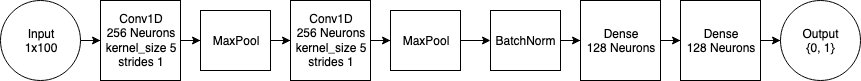
\includegraphics[width=\textwidth]{conv_architecture}
\centering
\end{figure}

\subsection{Fourier Convolutional Neural Network}
The Fourier Convolutional Neural Network leverages a custom "Fourier Layer", which moves the data into Fourier space via the Fast Fourier Transform before it performs a dot product on the input to the neuron.
Specifically, given an input $X^{(n)}$ and an output $A$, where the superscript is not an exponent, but instead indicates the layer of the input, the Fourier layer, $\ell$ acts on $X$:
\begin{align*}
X^{(n+1)} & = a \\
& = \ell^{(n)}(X^{(n)}) \\
& = \sigma(\mathcal{F}^{-1}(\mathcal{F}(X^{(n)})\cdot \mathbf{W}^{(n)\top}))
\end{align*}

Where $\mathcal{F}$ is the Fast Fourier Transform, $\sigma$ is the activation function - ReLU in this case - and $\mathbf{W}$ is the weight matrix for layer n.

Our Fourier ``Convolutional'' neural network is a mirror image of our standard convolutional neural network, only with the convolutional layers replaced by Fourier layers.
Here, we put the word convolutional in scare quotes due to the fact that no actual convolution is performed and thus it is a misnomer.
To be more intellectually honest, we should refer to this network instead as a ``Fourier Transform Inner Product Network'', though this may confuse readers unfamiliar with the relationship.
In the interest of broad understanding, the term convolutional neural network is used when it helps elucidate meaning even in spite of being a slight misnomer.

\subsection{Wavelet Convolutional Neural Network} \label{wavelet cnn}
The Wavelet Convolutional Neural Network implements similar functionality to our Fourier Neural Network, using the Continuous Wavelet Transform in lieu of the Fourier transform.
Due to the fact that there is a time component and a frequency component, the wavelet neural network has a higher dimensionality than our other models.

Details of the Wavelet Neural Network are pending a significant code revision.
This revision is due to some late work associated with the inversion of the continuous wavelet transform.

\subsection{Other Models} \label{other models}
Two baseline models were considered.
The first is the random forest model provided in the Scikit-learn library with no hyperparameter tuning.
Decision tree models are generally good at classification tasks~\cite{hastie01statisticallearning} but are weak classifiers which are sensitive to variance.
Random forests are a the result of averaging a large collection of de-correlated trees and provide a good benchmark as a na\"ive model - in the respect that it is untuned - for classification.

The other benchmark model is a Support Vector Classifier, again provided by the Scikit-learn library.
The rationale for using a Support Vector Machine is that we wanted to see if some hyperplane could be learned which would separate the data.
This model was again, na\"ive in the respect that it was merely the ``out of the box'' model, and so the classifier was built on top of the radial basis function kernel.
